% !TEX root= Thesis.tex
\chapter{Wire Segment Refinement}\label{chap:WireSegRefine}

  \begin{figure}[t]
    \centering
    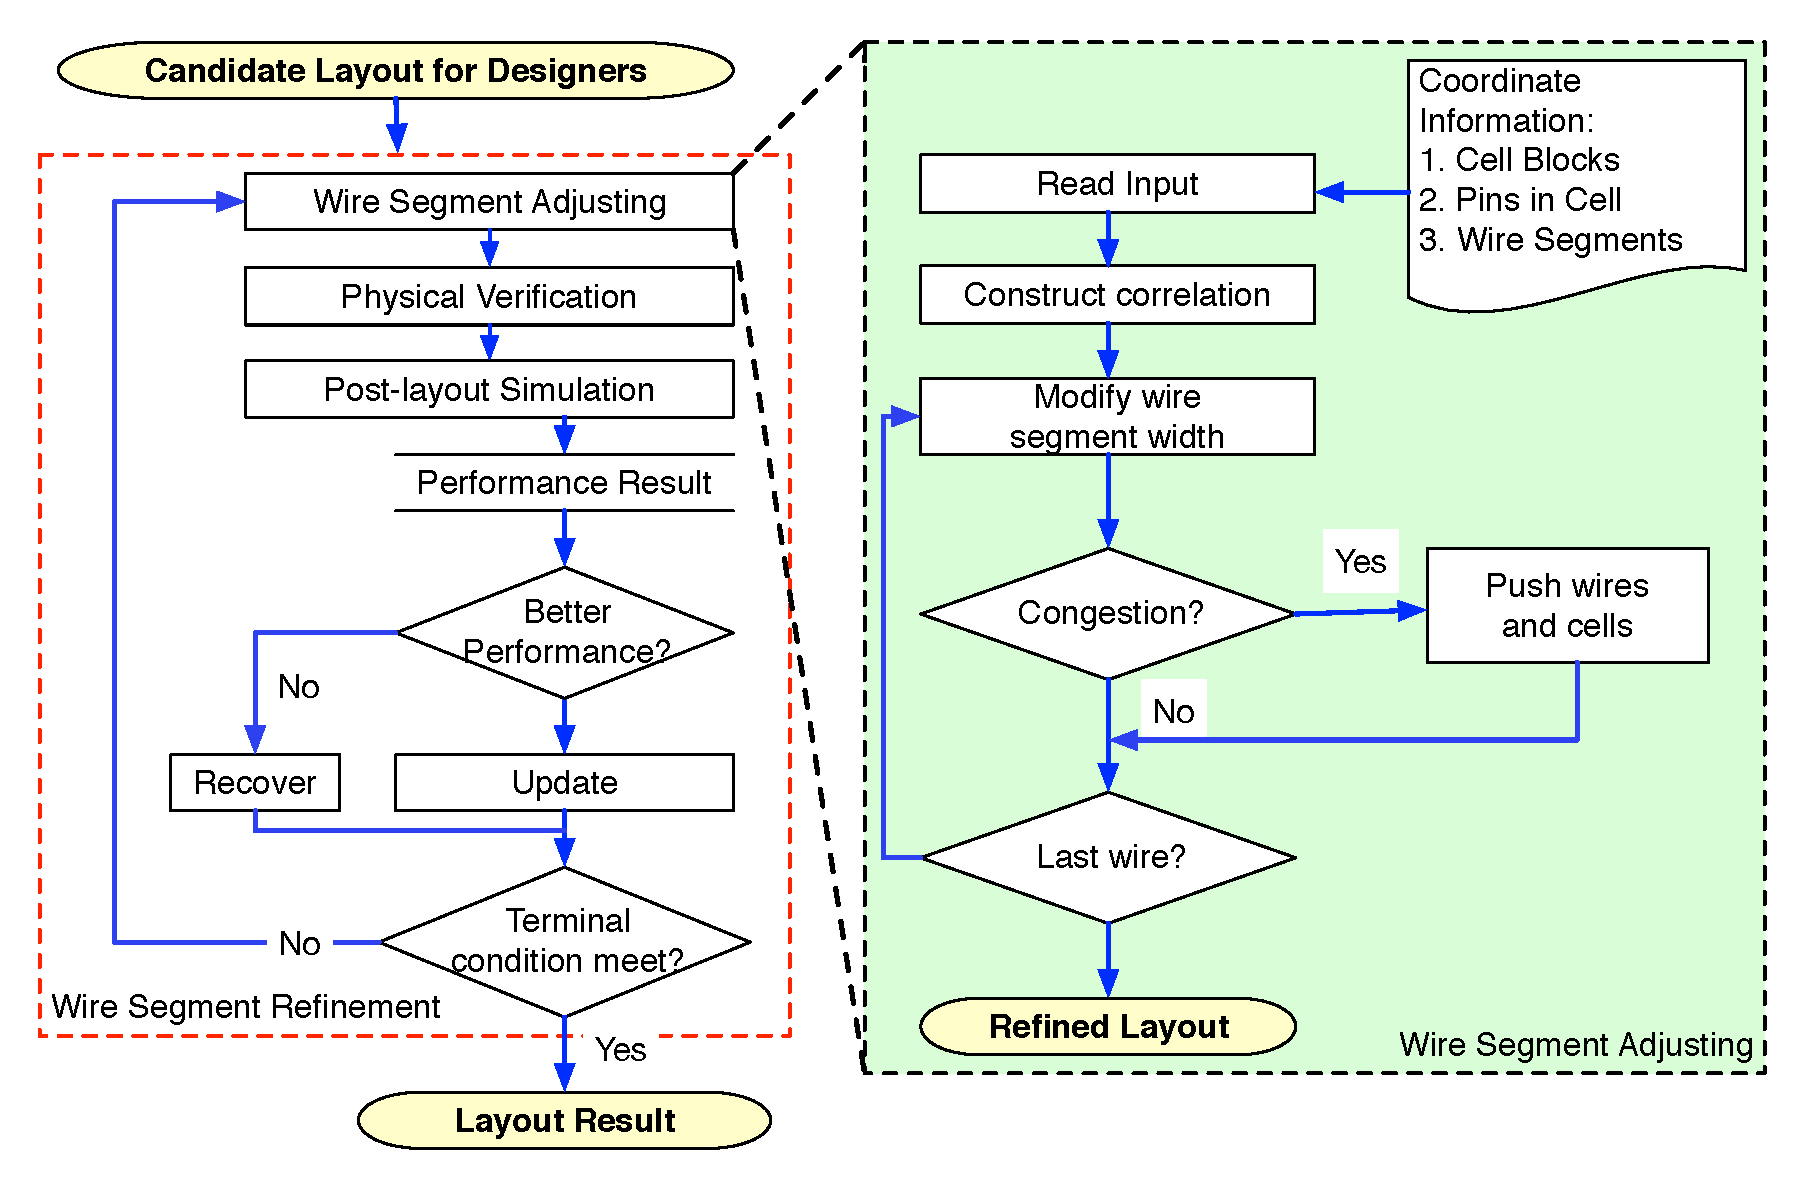
\includegraphics[width=\textwidth]{Fig/wireSegRefine.eps}
    \caption{Flow of the proposed Wire Segment Refinement.}
    \label{fig:WireSegRefine}
  \end{figure}
  
    


  After the prototypes of targeting layout is generated, these can be verified by design rules and post-layout simulation for manufacturing. In addition, our flow refines the routing on wire segments. Considering the resistant effect from wire segment, different width of each segment results in different unit resistance on routing. Practically speaking, the wires cannot be extended as wide as possible due to the limited area and design for manufacturing factors, which are relevant to advanced technologies. In this stage, our methodology traverses a solution under limited area with refined wire segments automatically. We practice a simulated annealing flow in Fig.~\ref{fig:WireSegRefine} to perturb the optimal solution for wire segments.

  
  

  According to {\it Wire Segment Adjusting} in Fig.~\ref{fig:WireSegRefine}, a set of segments is selected to change the width in each iteration and then the performance result is evaluated . Gathering the information of coordinate position and size of cell, every pin's location for each cell and the fixed block, is the prerequisite for the program. After having the information stored, finding the correlation of wires and cells becomes a chief task. The correlation should be established in horizontal and vertical respectively in each layer. For every layer, the routing wires are avoided overlapping on the cell area because of the possibility of crosstalk and unexpected error. The spaces left for horizontal (vertical) wires on upper and lower (left and right) directions are checked to obtain the preferred direction. Moreover, the trivial expansion of routing area can be avoided. 

  Later, we update the width of the targeting wire segment and then check the occurrence of any congestion. For every single step in simulated annealing, two wire segments are chosen randomly for updating. We increase one segment's width and decrease another. Since the area of the overall layout is fixed, the capacity for each segment is also limited. Changing the width of each wire segment makes congestion to be occurred easily. Once a congestion happens among blocks or wire segments, these wires or blocks are recursively pushed away from the congested area.

  Fig.~\ref{fig:Congestion} demonstrates one example for conducting the congestion elimination recursively. As soon as all the congestions are eliminated, the adjusting flow keeps changing the rest wires' width until there is no wire for adjusting. The refined layout with updated wire proceeds to physical verification. As the layout passing physical verification and the performance of such circuit is obtained by post-layout simulation. This layout is chosen based on possibility P which is related to the difference of the performance, the cooling-down temperature and the annealing factor to reduce the temperature. In the end, the layout with updated wires is generated.
  \begin{figure}[t]
    \centering
    \centerline{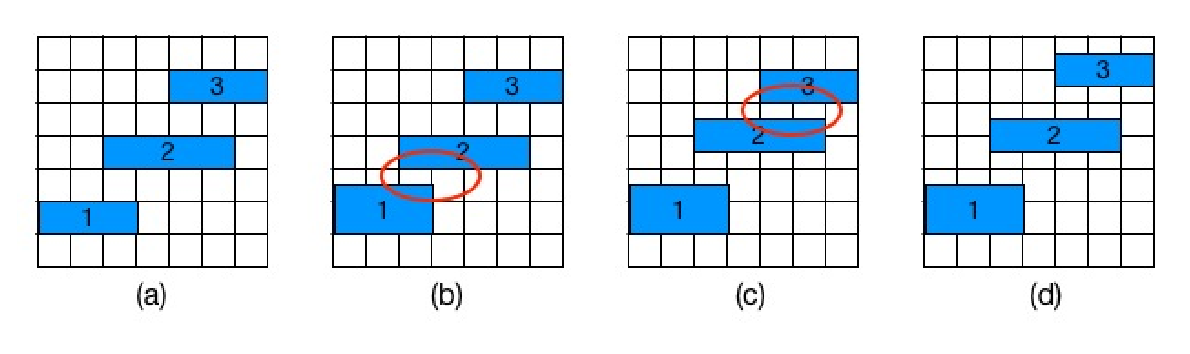
\includegraphics[width=\textwidth]{Fig/Congestion.eps}}
    \caption{Example of recursively segment pushing. (a) original layout. (b) Widened segment 1 and congestion occurs. (c) Pushing segment 2 above to avoid congestion between 1 and 2 but another congestion occurs among 2 and 3. (d) Pushing segment 3 above and then congestion eliminated.} 
    \label{fig:Congestion}
  \end{figure}